\documentclass[12pt]{beamer}

\usetheme[progressbar=frametitle]{metropolis}
\usepackage{appendixnumberbeamer}
\usepackage[numbers,sort&compress]{natbib}
\usepackage{caption}
\bibliographystyle{plainnat}
\usepackage[polish]{babel}
\usepackage{polski}
\usepackage{lmodern}
\usepackage{indentfirst}
\usepackage{booktabs}
\usepackage[scale=2]{ccicons}
\usepackage{xspace}

\newcommand{\themename}{\textbf{\textsc{metropolis}}\xspace}

\title{Organizacja pracy w grupie}
\date{2020}
\author{Zespół 9 - Paweł Bugyi, Marcin Michalski, Krzysztof Pierczyk}
\institute{Projektowanie układów sterowania (projekt grupowy)}


%-----------------------------------------------------------------------------%
%--------------------------------- Document ----------------------------------%
%-----------------------------------------------------------------------------%

\begin{document}

\maketitle

\begin{frame}{Agenda}
  \setbeamertemplate{section in toc}[sections numbered]
  \tableofcontents[hideallsubsections]
\end{frame}

\section{Przygotowanie do projektu, przydział zadań}
\label{podzial_zadan}

\begin{frame}<-7>[label=intro]{Wstępne przygotowania, przydział zadań}
    \centering
    \begin{itemize}
        \item<1-> Wykorzystane narzędzia (MATLAB, github, LaTeX, Jenkins, ...)
        \item<2-> Ściśle określona struktura drzewa projektowego
            \begin{enumerate}
                \item<3-> kod źródłowy
                \item<4-> konfiguracja projektu
                \item<5-> dokumentacja pomocnicza
                \item<6-> dokumentacja projektu
                \item<7-> ...
            \end{enumerate}
        \item<9-> Stały wzorzec dokumentacji
    \end{itemize} 
\end{frame}

\begin{frame}{Wstępne przygotowania, przydział zadań}
    \begin{figure}
        \centering
        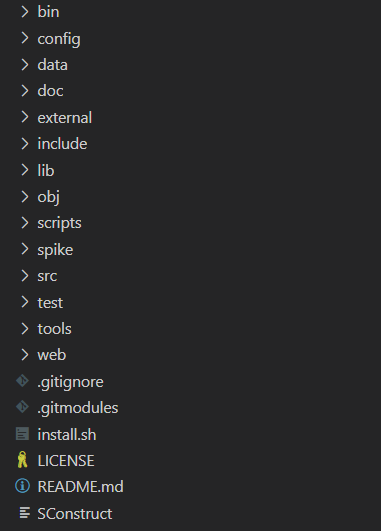
\includegraphics[scale=0.5]{img/project_tree.png}
        \caption{Przykładowe drzewo projektowe}
    \end{figure}
\end{frame}

\againframe<9->{intro}

\begin{frame}
    \frametitle{Nasz podział}
    \begin{itemize}[<+->]
        \item Napisanie kodu do zadania (MATLAB)
        \item Przeprowadzenie testów (MATLAB)
        \item Generacja sprawozdania (MATLAB, LaTeX)
    \end{itemize} 
\end{frame}
\section{Implementacja}

\begin{frame}<-5>[label=implementation]
    \frametitle{Implementacja}
    \begin{enumerate}
        \item<1-> Analiza teoretyczna
            \begin{itemize}
                \item<2-> jaki efekt chcemy osiągnąć?
                \item<3-> jakie mamy ograniczenia?
                \item<4-> jakich narzędzi możemy użyć?
            \end{itemize}
        \item<5-> Rozbicie zadania na podproblemy
        \item<6-> Ustalenie konwencji dotyczących tworzenia kodu
        \item<7-> Ciągłe testowanie oprogramowania
            \begin{itemize}
                \item<8-> testy jednostkowe
                \item<9-> scenariusze testowe
            \end{itemize}
    \end{enumerate} 
\end{frame}

\begin{frame}{Implementacja}
    \begin{figure}
        \centering
        
\includegraphics[scale=0.5]{img/modularity.png}
    \end{figure}
\end{frame}

\againframe<5-6>{implementation}

\begin{frame}{Implementacja}
    \begin{figure}
        \centering
        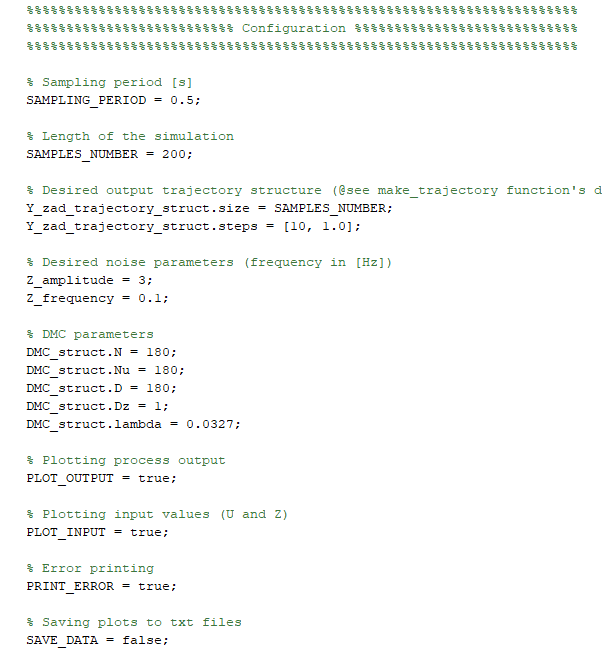
\includegraphics[scale=0.4]{img/Sekcja konfiguracyjna.PNG}
        \caption{Przykładowa sekcja konfiguracyjna}
    \end{figure}
\end{frame}

\againframe<6->{implementation}
\section{Wykonywanie eksperymentów}
\label{podzial_zadan}

\begin{frame}
    \frametitle{Eksperymenty}
    
    \begin{figure}[H]
    
\includegraphics[scale=0.5]{img/exp1.jpg} 
    \end{figure}
    
\end{frame}

\begin{frame}
    \frametitle{Przygotowanie scenariuszy testowych}
    \begin{figure}[!tbp]
      \centering
      \begin{minipage}[b]{0.4\textwidth}
        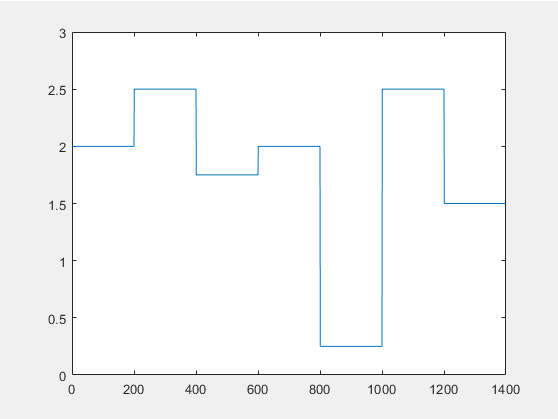
\includegraphics[scale = 0.35]{img/dobry_przebieg.PNG}
        \caption*{Dobry przebieg}
      \end{minipage}
      \hfill
      \begin{minipage}[b]{0.4\textwidth}
        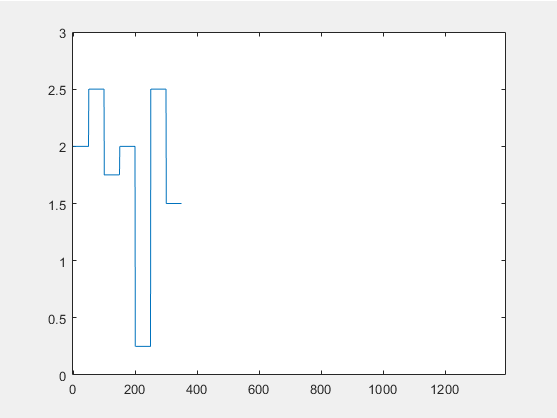
\includegraphics[scale = 0.35]{img/zly_przebieg.PNG}
        \caption*{Zły przebieg}
      \end{minipage}
    \end{figure}
\end{frame}

\begin{frame}
    \frametitle{Zautomatyzowanie testowania}
    \begin{figure}[H]
    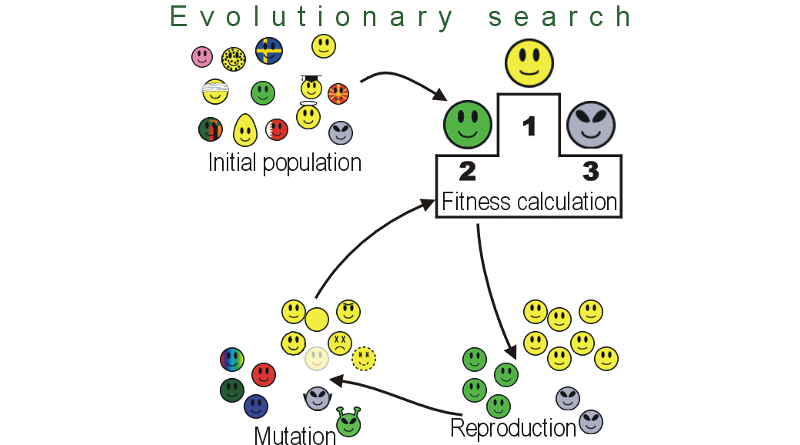
\includegraphics[scale=1.8]{img/algorytm_ewolucyjny.png} 
    \end{figure}
\end{frame}

\begin{frame}
    \frametitle{Przygotowanie się na potencjalne błędy podczas testowania}
    \begin{figure}[H]
    
\includegraphics[scale=0.3]{img/error.jpg} 
    \end{figure}
\end{frame}

\begin{frame}
    \frametitle{Podsumowanie części związanej z eksperymentami}
    \begin{figure}[H]
    
\includegraphics[scale=0.13]{img/chain.jpg} 
    \end{figure}
\end{frame}
\section{Opracowanie dokumentacji}

\begin{frame}
    \frametitle{Opracowanie dokumentacji}
    \begin{itemize}[<+->]
        \item Część teoretyczna sprawozdania
        \item Przygotowanie wykresów z danych wygenerowanyh w MATLABie
        \item Opis wyników
        \item Złożenie sprawozdania
    \end{itemize} 
\end{frame}

\subsection{Opracowanie dokumentacji}
\begin{frame}
    \frametitle{Generowanie wykresów }
    \begin{itemize}[<+->]
        \item Generowanie wykresów
            \begin{enumerate}
                \item     Tworzenie skryptów automatyzujących generację plików pdf 
                \item     Tworzenie skryptów automatyzujących generację kodu tworzącego wykresy w dokumentach 
                \item     Formatowanie wykresów w dokumentach 
            \end{enumerate}
    \end{itemize} 
\end{frame}

\begin{frame}
    \frametitle{Generowanie wykresów - przykłady }
    \begin{itemize}[<+->]
        \item Generowanie wykresów - nazewnictwo
            \begin{enumerate}
                \item     G1\_D\_180\_N\_60\_Nu\_25\_lambda\_25.txt
                \item     G1 D=180, N=60, $N_u$=25, $\lambda$=25
            \end{enumerate}
    \end{itemize} 
\end{frame}

\begin{frame}
    \frametitle{Tworzenie treści merytorycznej }
    \begin{itemize}[<+->]
        \item Tworzenie treści merytorycznej
            \begin{enumerate}
                \item     Analiza problemu 
                \item     Opis teoretyczny potencjalnych rozwiązań 
                \item     Analiza wyników 
                \item     Wnioski, zauważenie błędów, pomysły na poprawę w przyszłych projektach 
            \end{enumerate}
    \end{itemize} 
\end{frame}

\begin{frame}
    \frametitle{Formatowanie dokumentów }
    \begin{itemize}[<+->]
        \item Formatowanie dokumentów
            \begin{enumerate}
                \item     Dobór rozmiaru obrazów, dobór kolorystyki wykresów 
                \item     Rozmieszczenie obrazów z uwzględnieniem zachowania stałej gęstości teksu na stronie 
            \end{enumerate}
    \end{itemize} 
\end{frame}













\end{document}